\chapter{Problem Statement} \label{chap:chap3}

In this chapter the problem will be described and justified, using references from the bibliographic study presented in Chapter~\ref{chap:sota}.

\section{Problem Description}

Currently, FEUP's computing infrastructures are only accessed by those who have the technical knowledge to interact with the system. These people are technicians whose area of expertise encompasses outsourcing computing resources to perform computing jobs. 

If someone from an area unrelated to the computing system wants to perform any operation in it, that someone must contact the said technicians and waste valuable time for both parties cutting through red tape.

Having this in mind, CICA has started developing a project that reduces the ammount of knowledge necessary to perform the said computing operations.

This document focuses only on the front-end of the project, the back-end having already been developed by former MIEIC student Nuno Cardoso as part of his Master Thesis. CICA's project is described in greater detail in the following section.

\section{The project} \label{sec:project}


The project aims at simplifying the whole process and to make FEUP's computing infrastructures more accessible to the academic community, without the users having to spend time learning about the technologies and how the system actually works.

In order to better understand the full scope of the issue, Figure~\ref{fig:big_picture} shows the full system as it should function, through the means of an hypotetic and yet plausible use case scenario:

\begin{figure}[h!]
  \begin{center}
    \leavevmode
    \fbox{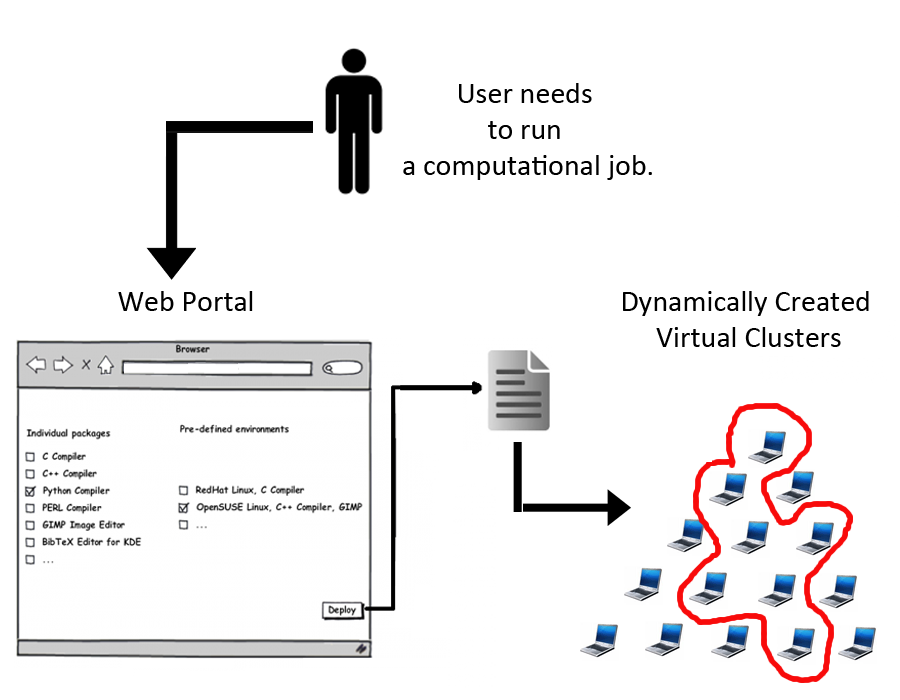
\includegraphics[width=\linewidth]{big_picture.png}}
    \caption{CICA's full computing project.}
    \label{fig:big_picture}
  \end{center}
\end{figure}

Firstly, a researcher of a specific field of study wants to conduct a more complex operation that involves greater computing efforts than his/her home and work computer. As such, the researcher proceeds to enter the designed system through a web page where he/she can:

\begin{itemize}
	\item Chose a suitable work environment for his/her computational needs according to a set of predefined parameters;
	\item Create his/her own work environment according to the specifications he/she provides the system with.
\end{itemize}

The system will then automatically create a virtual environment (image containing all the information needed), which will be passed onto the back-end of the project where a virtual cluster will be created according to that virtual environment.
Finally a username and password combination should be returned so that the researcher can enter the created environment and perform his/her operations. 

The objectives for this project can be divided as following:

\begin{enumerate}
\item Implementing the creation of virtual images;
\item Making the creation according to what the users specify --- image contextualization;
\item Passing the images created to \textit{OpenStack}. This includes connecting with both \textit{Horizon}(dashboard) and \textit{Glance} (image service).
\item Creating a web system that makes the objectives above transparent for the user.
\end{enumerate}


\section{The solution}\label{sec:solution}

As mentioned in the above section, one of the main objectives of this dissertation is the integration of an \textit{OpenStack} --- presented in Chapter~\ref{chap:sota} --- deployment environment as it should simplify the cloud creation and management. 

In this section of this chapter the technological choices are presented and justified.

\subsection{The chosen technologies}\label{subsec:tech}

One thing was missing in the cloud computing scene... A cloud management layer. A cloud operating system that added automation and control at scale. That is where \textit{OpenStack} comes into play. As mentioned in Chapter~\ref{chap:sota}, section~\ref{subsec:openstack} it is built by a world wide community of developers, something that made it a good choice to investigate, as the open source culture is something always worthy of enriching.~\cite{stackgithub}

There is one thing one must keep in mind: as it was described in Chapter~\ref{chap:sota}, \textit{OpenStack} is not the only solution available. \textit{OpenNebula} was also available and is already up and running at FEUP. So why choose \textit{OpenStack}?

First of all, \textit{OpenStack} is a more recent project and \textit{OpenNebula}. It is backed up by some renowned names in the industry, such as \textit{Dell}, \textit{AMD}, \textit{Intel}, \textit{Canonical}, \textit{Cisco}, \textit{StackOps}, \textit{HP}, \textit{NEC}, \textit{AT \& T}, \textit{Yahoo!} and \textit{Red Hat}. Some of these companies also support \textit{OpenNebula}.

The coding activity on both projects was also taken into account when chosing which to deploy. With the help of OHLOH~\footnote{An open source directory that anyone can edit. It features comprehensive metrics and analysis on thousands of open source projects.~\cite{ohloh}}, the differences can be easily observed as it is shown in Figure~\ref{fig:ohloh_compare}, which is included in Appendix~~\ref{chap:ap2}.

\textit{OpenStack} has more favourable statistics, such as the number of committers and number of commits (shown in Figures~\ref{fig:committers} and~\ref{fig:commits}) over time. If this is viewed with the knowledge that \textit{OpenNebula} was created first, and \textit{OpenStack} managed to outdo it, great things can be expected.

\begin{figure}[h]
  \begin{center} 
    \leavevmode 
    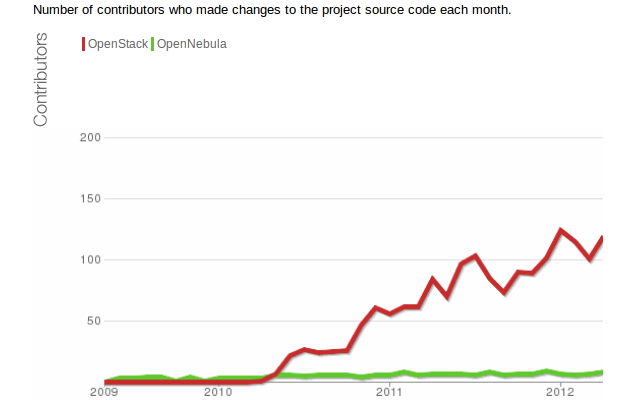
\includegraphics[scale=0.65]{committers}
    \caption{Comparison between the number of committers on \textit{OpenStack} and \textit{OpenNebula}.~\cite{ohloh}} 
    \label{fig:committers} 
  \end{center}
\end{figure}

\begin{figure}[h]
  \begin{center}
    \leavevmode
    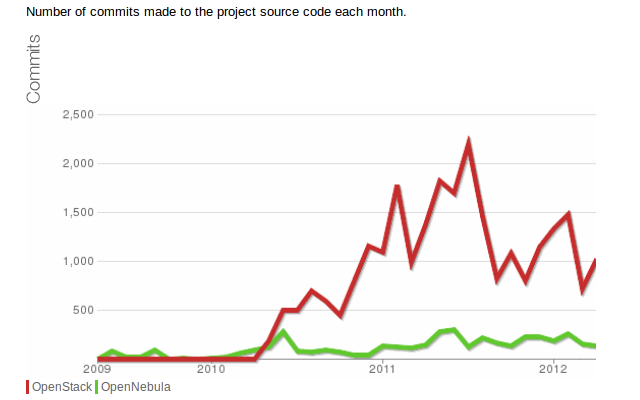
\includegraphics[width=\textwidth]{commits}
    \caption{Comparison between the number of commits on \textit{OpenStack} and \textit{OpenNebula}.~\cite{ohloh}}
    \label{fig:commits}
  \end{center}
\end{figure}

In addition to this and as it was refered in Chapter~\ref{chap:sota}, section~\ref{subsec:opennebula}, \textit{OpenNebula}'s creators have founded an enterprise of their own (C12G Labs) which offers an enterpreise version of \textit{OpenNebula} (named \textit{OpenNebulaPro}). This deviates from the open source philosophy, something that \textit{OpenStack} maintains.

On a more technical aspect, \textit{OpenStack} is mainly written in \textit{Python} whereas \textit{OpenNebula} is mainly coded in \textit{C++} and \textit{Ruby}, as it can be observed in Figure~\ref{fig:code-stack-nebula}. 

In order to understand the relevance of this detail, it must be said that there is an extensive and obligatory contact with \textit{C++} in MIEIC, something that does not happen with \textit{Ruby}, and \textit{Python} is not presented at all. Previous experience with both \textit{C++} and \textit{Ruby} proved to be unfulfilling (\textit{C++} due to its not-so-high-level nature and \textit{Ruby} because it was used in the context of \textit{Ruby on Rails}, which due to some installation quirks was deemed impossible to start and use). 

\textit{Python} on the other hand, was a different programming language, something that was going to be a challenge. Coupled with \textit{Django}, it promised the same advantages as \textit{Ruby on Rails}, but with less trouble getting it up and running. Since \textit{Horizon} is built on \textit{Django}, the choice seemed obvious. The cherry on top of the cake would be contributing to FEUP's knowledge on the new technologies to be researched (\textit{Django}, \textit{Python} and of course, \textit{OpenStack}).

The previous experience with \textit{Ruby} paired with the desire for new challenges and learning new programming languages, \textit{OpenStack} was chosen. This would also allow to contribute to FEUP's knowledge on this new technology.

\begin{figure}[h!]
  \begin{center}
    \leavevmode
    \fbox{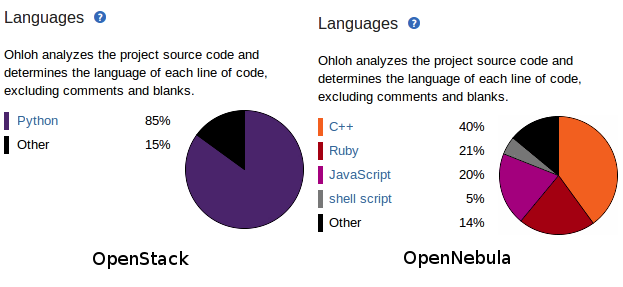
\includegraphics[scale=0.5]{code-stack-nebula}}
    \caption{Comparison between the programming languages in \textit{OpenStack} and \textit{OpenNebula}.~\cite{ohloh}}
    \label{fig:code-stack-nebula}
  \end{center}
\end{figure}

Rodrigo Benzaquen, director of site operations and infrastructure at MercadoLibre, a Latin America e-commerce market leader which chose to use \textit{OpenStack} as their cloud solution, stated the following:

\begin{quote}
 ``Before this [\textit{OpenStack}'s deployment], we would have had someone physically deploy the server which would take a day or longer. With \textit{OpenStack}, we don't have to do that; our developers are now able to create and manage their servers.''\cite{openstack-userstories}
\end{quote}

which came directly into the objective of this dissertation, easing the cloud creation and management process.

\clearpage
\subsection{Connecting the dots}\label{subsec:architecture}

As mentioned in Chapter~\ref{chap:sota}, section~\ref{subsec:openstack}, \textit{OpenStack} is designed to deliver a massively scalable cloud operating system, each of the components being designed to work together in order to prodive complete IaaS. This integration is facilitated through pulic APIs that each service offers, being available to the cloud's end users.~\cite{ken-pepple:essex-arch}. 

Expanding the diagram shown in Figure~\ref{fig:openstack_sw_diag}, the relationships between the services are shown in Figure~\ref{fig:openstack_services}:

\begin{figure}[h!]
  \begin{center}
    \leavevmode
    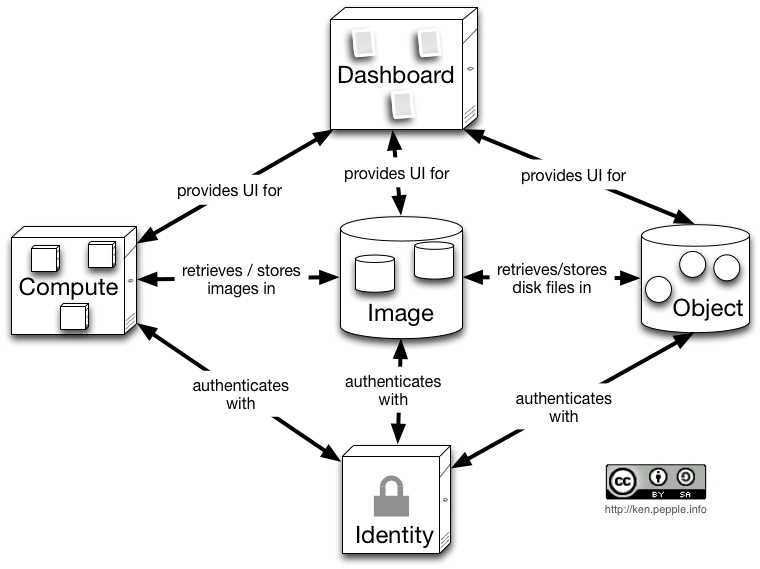
\includegraphics[scale=0.5]{nova-concept-int-essex}
    \caption{Relationships between the different \textit{OpenStack} services.~\cite{ken-pepple:essex-arch}}
    \label{fig:openstack_services}
  \end{center}
\end{figure}

The solution proposed for this project links the \textit{OpenStack} Dashboard --- \textit{Horizon} --- with the designed \textit{Web application} developed in \textit{Python} and \textit{Django}, as shown in Figure~\ref{fig:architecture}.

\begin{figure}[t]
  \begin{center}
    \leavevmode
    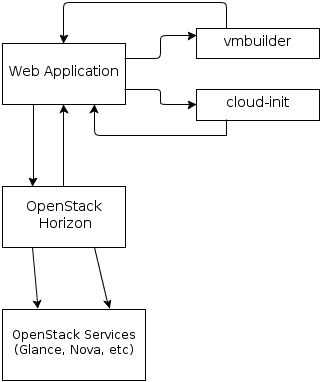
\includegraphics[scale=0.5]{architecture}
    \caption{Proposed architecture implementation.}
    \label{fig:architecture}
  \end{center}
\end{figure}

As it can be observed, the web application will use \texttt{vmbuilder} and \textit{cloudinit} whenever needed and then passing that information to the \textit{OpenStack Horizon} dashboard, which will communicate with the rest of \textit{OpenStack} services.

Since \texttt{vmbuilder} and \textit{cloudinit} work for different purposes (\texttt{vmbuilder} creates contextualized VM images and \textit{cloudinit} contextualizes clean VM images), different tools will be used for different purposes.



An interesting feature to complete in future work could be eliminating the web system and passing the image creation and contextualization to \textit{OpenStack}, modifying the \textit{Horizon} dashboard itself.
 

%Este capítulo deve começar por fazer uma apresentação detalhada do
%problema a resolver\footnote{Na introdução a apresentação do
%  problema foi breve.} podendo mesmo, caso se justifique,
%constituir-se um capítulo com essa finalidade.

%Deve depois dedicar-se à apresentação da solução sem detalhes de
%implementação. 
%Dependendo do trabalho, pode ser uma descrição mais teórica, mais
%``arquitectural'', etc.
%\clearpage
\section{Conclusions}

In this chapter was presented the architecture to be followed in Chapter~\ref{chap:chap4} in the implementation phase of the project. The objectives were also outlined, as well as which technologies to use.
